\documentclass{beamer}
\usetheme{Copenhagen}
\usepackage{hyperref}
\usepackage[T1]{fontenc}

% other packages
\usepackage{latexsym,amsmath,xcolor,multicol,booktabs,calligra}
\usepackage{graphicx,pstricks,listings,stackengine}

\author{Andrei Ilin}
\title{Timing Anomaly through Branch Prediction}
% \subtitle{Cospa group meeting}
\subtitle{Supervised by Lionel Rieg, Florian Brandner and Mihail Asavoae}
\institute{Université Grenoble Alpes}
\date{23 June 2025}
\usepackage{USTC_beamer}

% \renewcommand{\familydefault}{\rmdefault}

% defs
\def\cmd#1{\texttt{\color{red}\footnotesize $\backslash$#1}}
\def\env#1{\texttt{\color{blue}\footnotesize #1}}
\definecolor{deepblue}{rgb}{0,0,0.5}
\definecolor{deepred}{rgb}{0.6,0,0}
\definecolor{deepgreen}{rgb}{0,0.5,0}
\definecolor{halfgray}{gray}{0.55}

\lstset{
    basicstyle=\ttfamily\small,
    keywordstyle=\bfseries\color{deepblue},
    emphstyle=\ttfamily\color{deepred},  
    stringstyle=\color{deepgreen},
    numbers=left,
    numberstyle=\small\color{halfgray},
    rulesepcolor=\color{red!20!green!20!blue!20},
    frame=shadowbox,
}


\begin{document}

% \kaishu
\renewcommand{\figurename}{Fig.}

% logo
\begin{frame}
    \titlepage
    \begin{figure}[htpb]
        \begin{center}
            
\includegraphics[width=0.2\linewidth]{pic/logo-uga.png}\hspace{1.5cm}
            
\includegraphics[width=0.2\linewidth]{pic/logo-verimag.png}\hspace{1.5cm}
            
\includegraphics[width=0.2\linewidth]{pic/logo-INP.png}
        \end{center}
    \end{figure}
\end{frame}

\begin{frame}
    \tableofcontents[sectionstyle=show,subsectionstyle=show/shaded/hide,subsubsectionstyle=show/shaded/hide]
\end{frame}

\section{Introduction}

\begin{frame}{Critical Real-Time Systems}
    \begin{columns}
        \begin{column}{0.5\textwidth}
            \begin{block}{Can be found in:}
                \begin{itemize}
                    \item Cars 
                    \item Planes
                    \item Life-supporting equipment
                \end{itemize}
            \end{block}
        \end{column}

        \begin{column}{0.5\textwidth}
            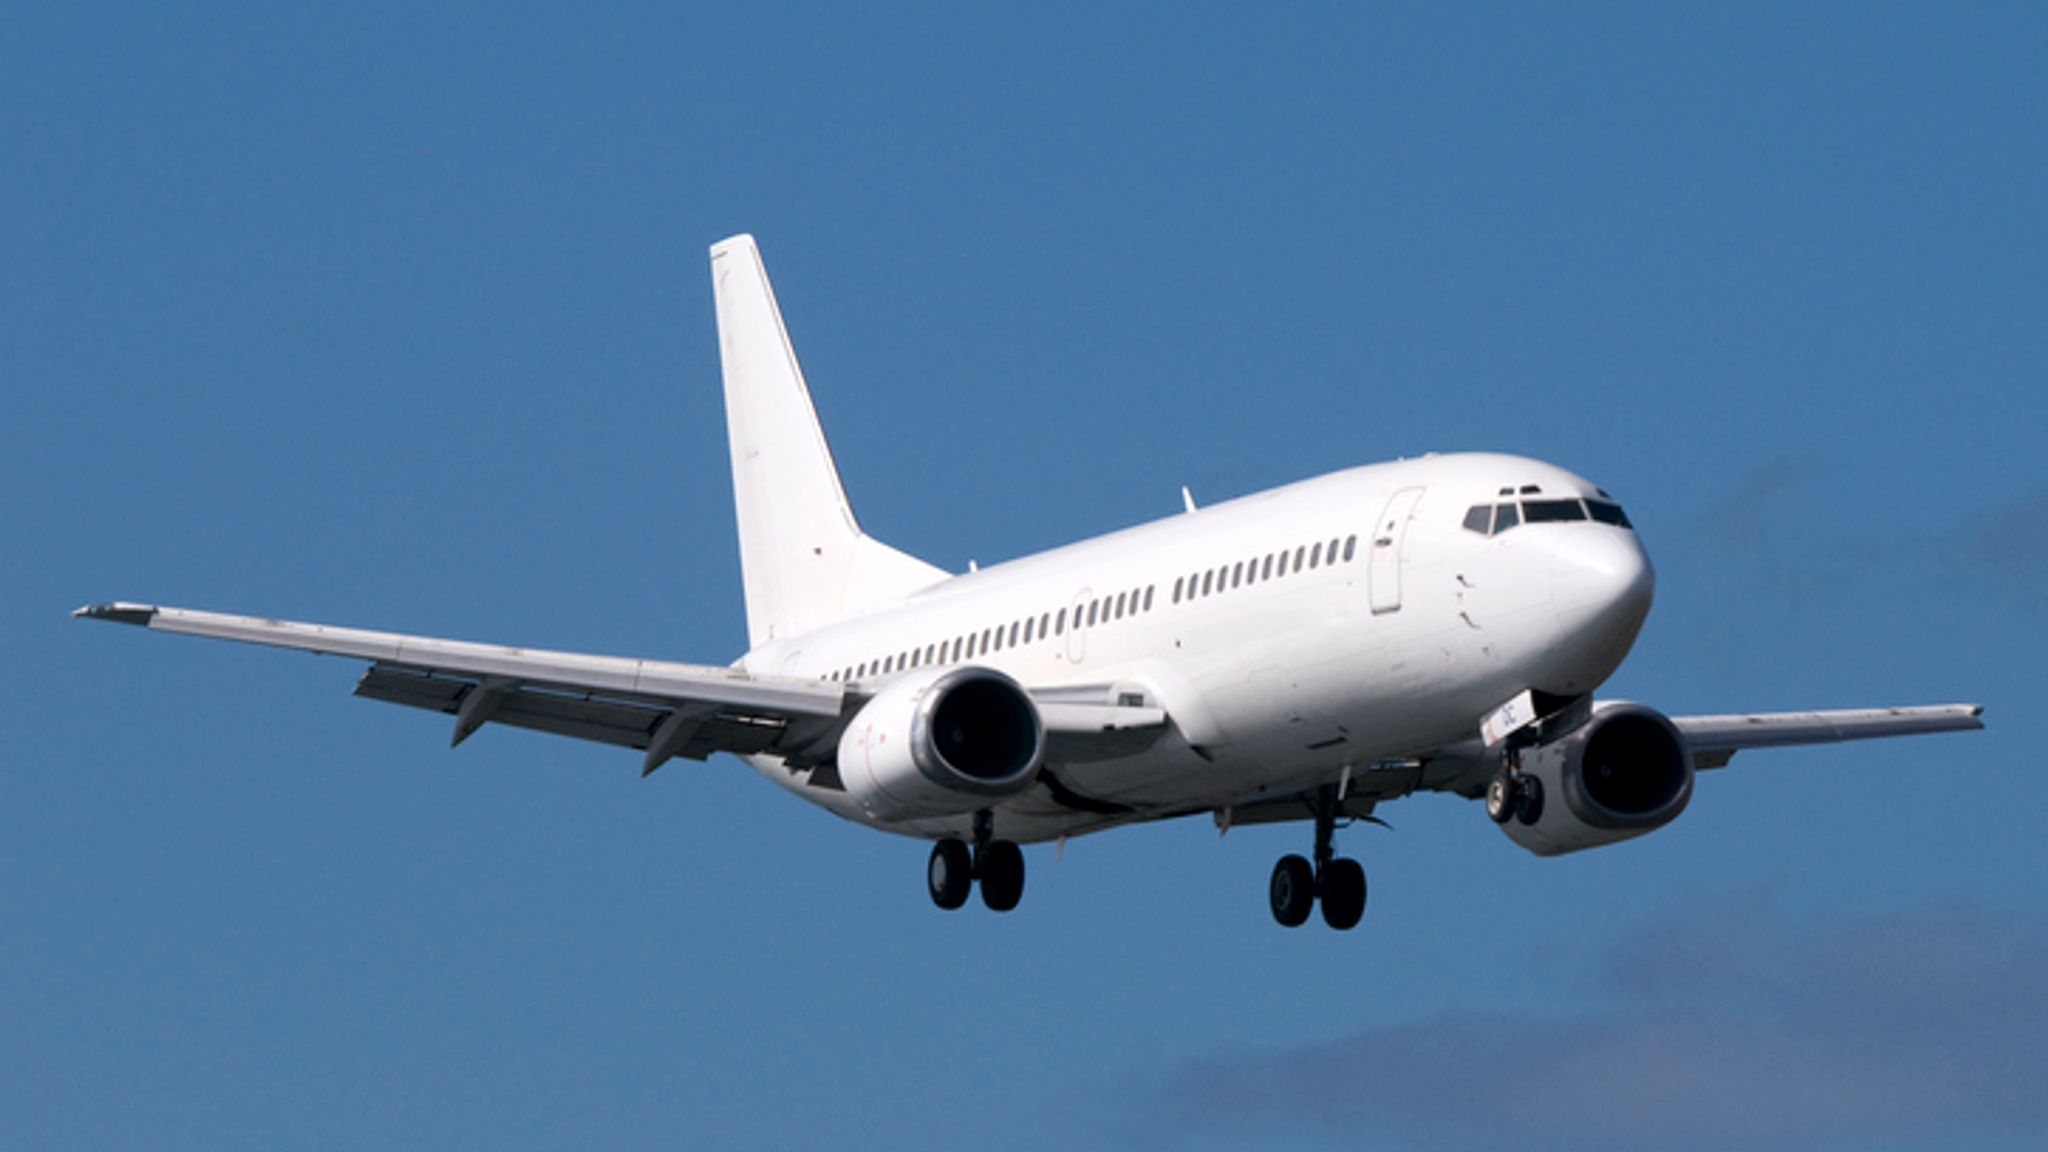
\includegraphics[width=\textwidth]{pic/plane.png}
        \end{column}
    \end{columns}

    \hfill \break
    \hfill \break

    Critical Real-Time Systems are expected to finish on time, otherwise the disaster could happen. This often requires special hardware and software that can be analyzed for timing properties.
    
\end{frame}


\begin{frame}{WCET Analysis}
    \begin{columns}
        
    \column{0.4\textwidth}

    \textbf{W}orst \textbf{C}ase \textbf{E}xecution \textbf{T}ime Analysis:
    \begin{itemize}
        \item Hardware + Software $\downarrow$
        \item Upper bound for execution time?
    \end{itemize}


    \begin{block}{}
        Using abstract execution models. Split analysis into phases related to SW and HW parts.
    \end{block}

    \column{0.6\textwidth}

    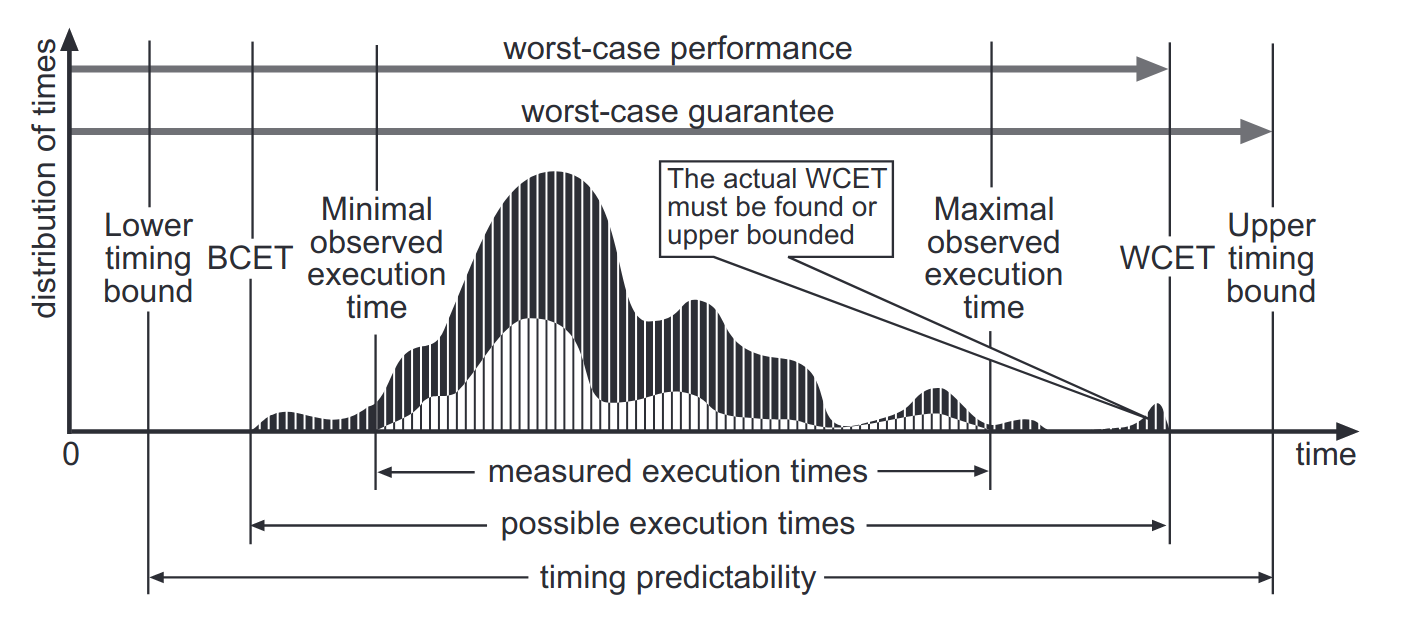
\includegraphics[width=1\textwidth]{pic/timing-distribution.png}

    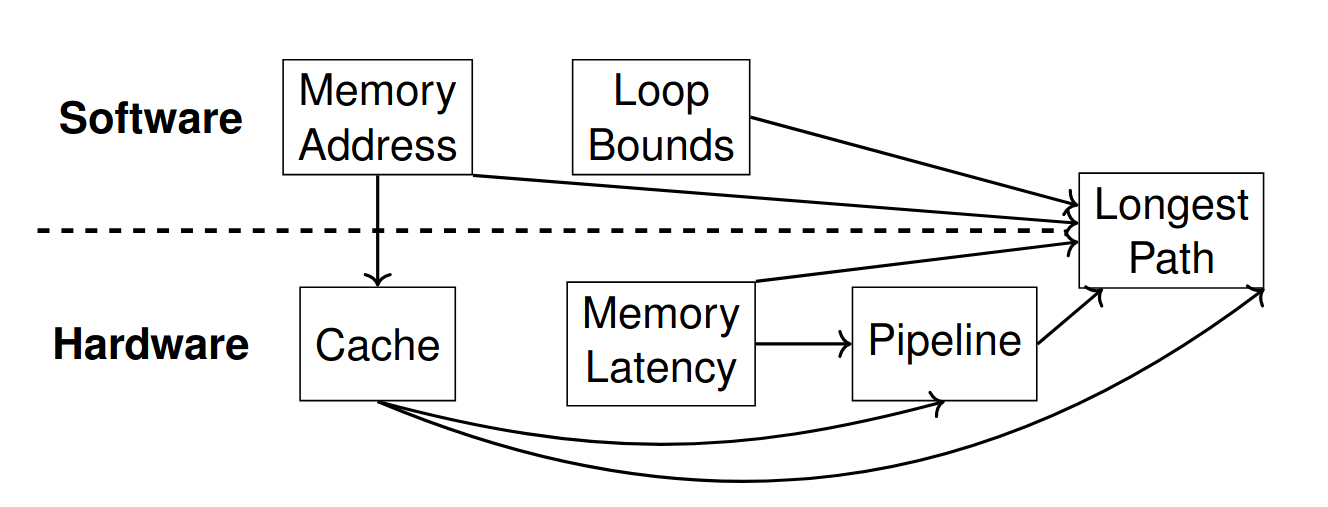
\includegraphics[width=1\textwidth]{pic/wcet-deps.png}

    \end{columns}
\end{frame}

\begin{frame}{Timing Anomalies}
    \begin{block}{Timing Anomaly (TA)}
        When a local speedup leads to a global slowdown.
    \end{block}

    \begin{exampleblock}{Example}
        Faster completion of $A$ leads to a slowdown of the whole trace. 
    \end{exampleblock}

    \begin{columns}
    \column{0.4\textwidth}
        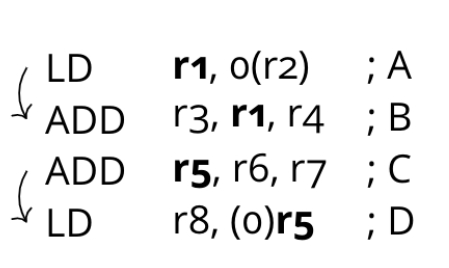
\includegraphics[width=1\textwidth]{pic/first-TA-ex-input.png}
    \column{0.6\textwidth}
        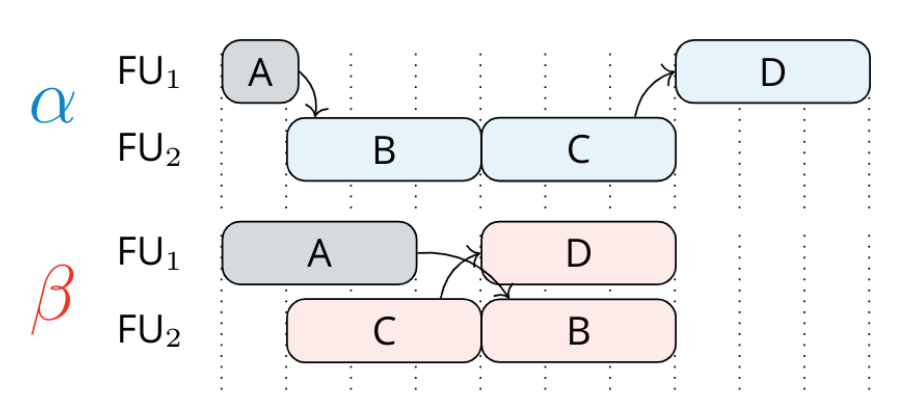
\includegraphics[width=1\textwidth]{pic/first-TA-ex-trace.png}
    \end{columns}
    
\end{frame}
    
\section{Hardware}

\begin{frame}{OoO Multiscalar Pipeline}
    Processor:
    \begin{itemize}
        \item \textbf{Pipelined:} Divided into consecutive stages
        \item \textbf{Multiscalar:} Fetch multiple instruction in the same time
        \item \textbf{Out-of-Order:} Execution order dictated by instruction dependencies
    \end{itemize}


    \begin{columns}
    \column{0.5\textwidth}
        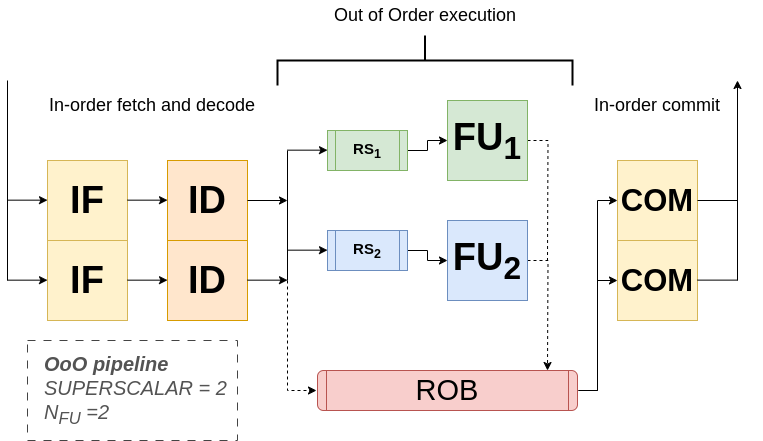
\includegraphics[width=\textwidth]{pic/ooo-pipeline.png}
    \column{0.5\textwidth}
        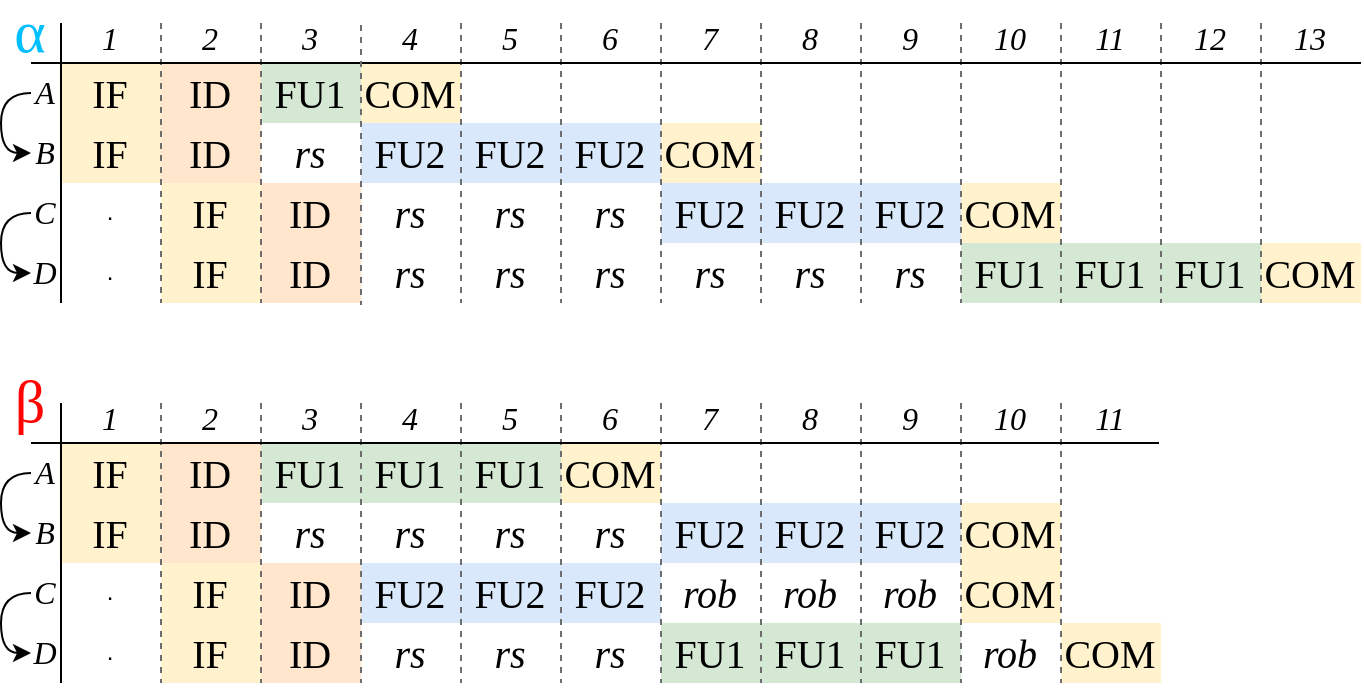
\includegraphics[width=\textwidth]{pic/multiscalar_ta.png}
    \end{columns}

\end{frame}

\begin{frame}{Branch Prediction}
    
\end{frame}

\begin{frame}{Branch Prediction: possible implementations}
    
\end{frame}

\section{Timing Anomalies}

\section{Contribution}

\section{Conclusion}

\end{document}
